% ============================================================
%  Trebuchet Build Guide -- generic, any scale
%  Forces & Motion (Yr 7-8). Every size is a multiple of L,
%  the throwing-arm length (pivot to release pin).
%  Compile: pdflatex Trebuchet_Build_Guide.tex (twice)
% ============================================================
\documentclass[11pt,a4paper]{article}
\usepackage[T1]{fontenc}

\usepackage[a4paper, top=1.2cm, bottom=1.6cm, left=1.5cm, right=1.5cm]{geometry}
\usepackage{xcolor}
\usepackage{tikz}
\usetikzlibrary{arrows.meta,calc,patterns,decorations.pathreplacing,decorations.markings}
\usepackage{booktabs}
\usepackage{array}
\usepackage{tabularx}
\usepackage{enumitem}
\usepackage{amsmath}
\usepackage{fancyhdr}
\usepackage[protrusion=true,expansion=false]{microtype}

% ── Colours (muted, print-friendly) ─────────────────────────────────────────
\definecolor{Ink}      {HTML}{1A1A1A}
\definecolor{HeadGrey} {HTML}{333333}
\definecolor{RuleGrey} {HTML}{888888}
\definecolor{BoxGrey}  {HTML}{F0F0F0}
\definecolor{LineGrey} {HTML}{555555}
\definecolor{WarnBg}   {HTML}{F5F5F5}
\definecolor{Wood}     {HTML}{E2CFA8}
\definecolor{WoodDark} {HTML}{B8996A}
\definecolor{Steel}    {HTML}{6B7178}
\definecolor{Plate}    {HTML}{9AA0A6}

\setlength{\parindent}{0pt}
\setlength{\parskip}{3pt}
\renewcommand{\arraystretch}{1.2}

\newcolumntype{L}[1]{>{\raggedright\arraybackslash}p{#1}}
\newcolumntype{C}[1]{>{\centering\arraybackslash}p{#1}}
\newcolumntype{Y}{>{\raggedright\arraybackslash}X}

\newcommand{\sechead}[1]{%
  \par\vspace{6pt}%
  {\bfseries\large\color{HeadGrey} #1}\\[-4pt]
  {\color{RuleGrey}\rule{\linewidth}{0.8pt}}\par\vspace{1pt}
}
\newcommand{\step}[2]{\par\vspace{4pt}{\bfseries\color{Ink} Step #1 --- #2}\par}

\newcommand{\warnbox}[1]{%
  \par\vspace{3pt}\noindent
  \fcolorbox{LineGrey}{WarnBg}{\parbox{\dimexpr\linewidth-2\fboxsep-2\fboxrule}{\small #1}}\par\vspace{3pt}}

\pagestyle{fancy}
\fancyhf{}
\renewcommand{\headrulewidth}{0pt}
\fancyfoot[L]{\footnotesize\color{RuleGrey} Trebuchet Build Guide \textbullet{} Forces \& Motion, Year 7--8}
\fancyfoot[R]{\footnotesize\color{RuleGrey} Page \thepage}

% ── TikZ styles ─────────────────────────────────────────────────────────────
\tikzset{
  dim/.style={{Stealth[length=4pt]}-{Stealth[length=4pt]}, thin, Ink},
  ext/.style={very thin, RuleGrey},
  lbl/.style={font=\scriptsize, text=Ink, align=left},
  lead/.style={thin, LineGrey},
  dl/.style={font=\scriptsize, fill=white, inner sep=1pt, text=Ink},
  wood/.style={fill=Wood, draw=Ink, thin},
  steel/.style={fill=Steel, draw=Ink, thin},
  % the arm, drawn along local +x and rotated about the pivot.
  % local +y is the sling side.
  pics/arm/.style={code={
    \fill[Plate, opacity=0.55, draw=Ink, thin] (-0.25,0) circle (0.14);
    \fill[Wood, draw=Ink, thin] (-0.30,-0.035) -- (0.05,-0.035) -- (1.0,-0.0175)
      -- (1.0,0.0175) -- (0.05,0.035) -- (-0.30,0.035) -- cycle;
    \fill[Steel, draw=Ink, very thin] (-0.25,0) circle (0.016);
    \draw[Steel, line width=1.1pt] (1.0,0) -- (1.05,0);
    \fill[white, draw=Ink, thin] (0,0) circle (0.022);
  }},
  pics/frame/.style={code={
    % base rail, legs and bearing block, side view, base top at y = 0
    \fill[WoodDark, draw=Ink, thin] (-0.80,-0.06) rectangle (0.70,0);
    \draw[Ink, line width=0.4pt, fill=Wood] (-0.37,0) -- (-0.33,0) -- (0.02,0.84) -- (-0.02,0.84) -- cycle;
    \draw[Ink, line width=0.4pt, fill=Wood] (0.33,0) -- (0.37,0) -- (0.02,0.84) -- (-0.02,0.84) -- cycle;
    \fill[WoodDark, draw=Ink, thin] (-0.06,0.79) rectangle (0.06,0.90);
    % trough
    \fill[BoxGrey, draw=Ink, very thin] (-0.70,0) rectangle (0.50,0.03);
  }},
}

\begin{document}
\small

% =====================================================================
%  PAGE 1 -- HOW IT WORKS
% =====================================================================
{\LARGE\bfseries\color{Ink} Trebuchet Build Guide --- any scale}\\[3pt]
{\color{RuleGrey}\rule{\linewidth}{1.2pt}}

This guide builds a counterweight trebuchet at any size, from a desktop model to one that throws a tennis ball 20--30\,m across an oval. \textbf{Every measurement is a multiple of one number, $L$}: the length of the throwing arm, from the centre of the pivot to the release pin. Pick $L$, multiply, and cut. Page~2 has the sizes already worked out for three scales.

\sechead{How it works}
A heavy counterweight on the short arm falls and swings the long throwing arm up and over. The sling, hanging from the tip of the arm, whips round faster still. One end of the sling is a loop resting on the release pin: when the sling swings far enough round, the loop slides off and the projectile flies free. A tennis ball can leave at two to three times the speed of the arm's tip.

\begin{center}
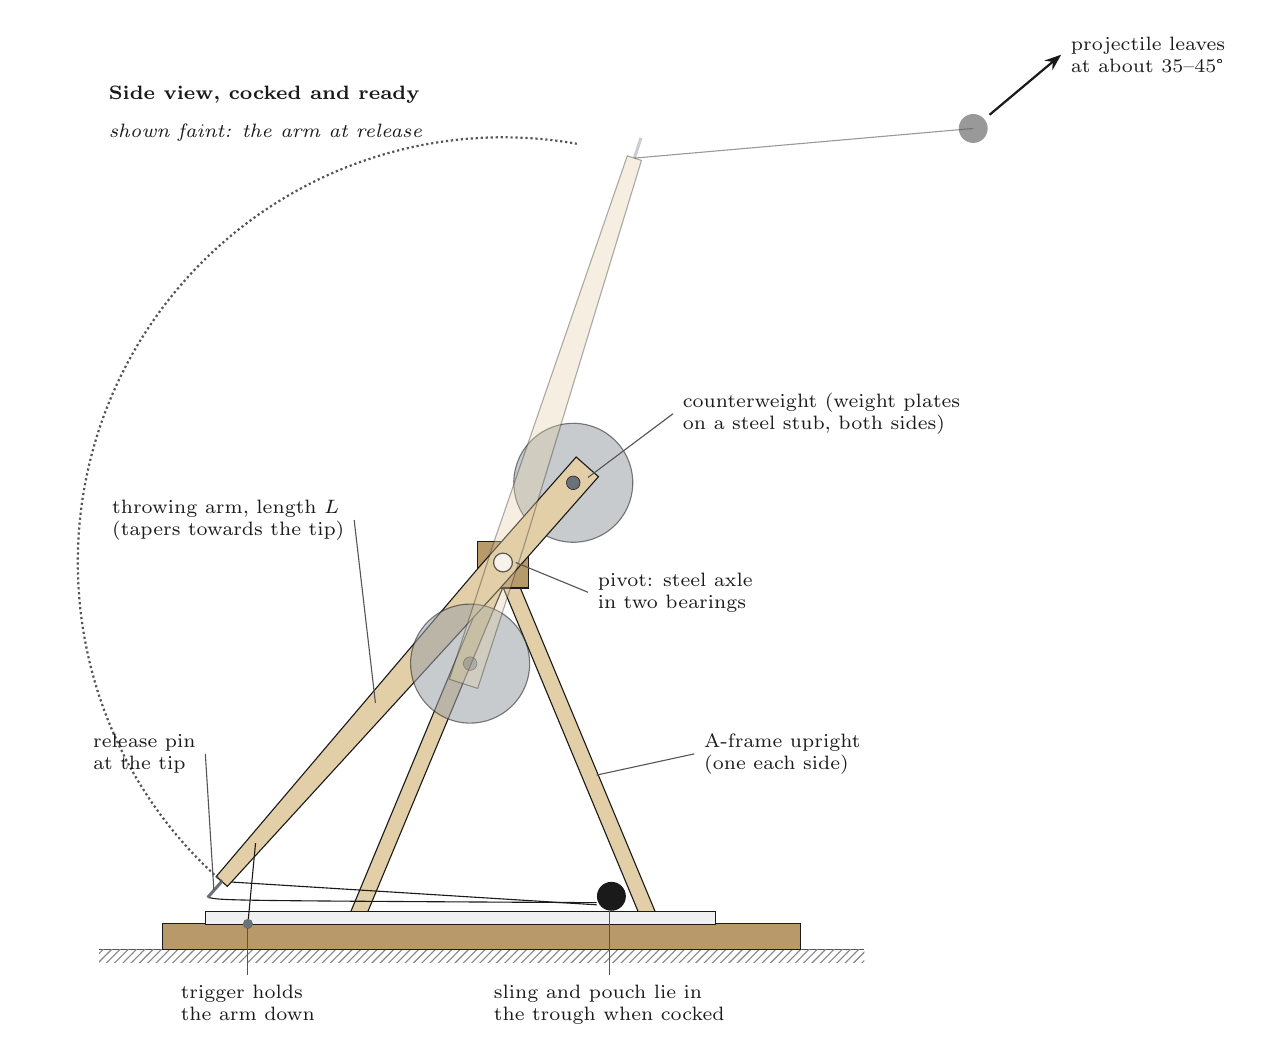
\begin{tikzpicture}[x=5.4cm, y=5.4cm]
  % ground
  \draw[LineGrey] (-0.95,-0.06) -- (0.85,-0.06);
  \fill[pattern=north east lines, pattern color=RuleGrey] (-0.95,-0.09) rectangle (0.85,-0.06);
  \pic at (0,0) {frame};
  % sling along the trough, ball in pouch
  \coordinate (T) at ($(0,0.85)+(228.6:1)$);
  \draw[Ink, thin] (T) -- (0.22,0.045);
  \draw[Ink, thin] ($(T)+(228.6:0.05)$) .. controls (-0.66,0.055) .. (0.22,0.05);
  \fill[Ink] (0.255,0.065) circle (0.034);
  % arm, cocked
  \pic[rotate=228.6] at (0,0.85) {arm};
  % trigger
  \draw[Ink, thin] ($(0,0.85)+(228.6:0.88)$) -- (-0.60,0);
  \fill[Steel] (-0.60,0) circle (0.012);
  % ghost: arm at release
  \draw[densely dotted, LineGrey, thick] ($(0,0.85)+(228.6:1)$) arc[start angle=228.6, end angle=80, radius=1];
  \begin{scope}[opacity=0.35]
    \pic[rotate=72] at (0,0.85) {arm};
  \end{scope}
  \coordinate (Tr) at ($(0,0.85)+(72:1)$);
  \draw[LineGrey, thin, opacity=0.6] (Tr) -- ++(5:0.80) coordinate (B);
  \fill[LineGrey, opacity=0.6] (B) circle (0.034);
  \draw[-{Stealth[length=6pt]}, thick, Ink] ($(B)+(40:0.05)$) -- ++(40:0.22);
  \node[lbl, anchor=west] at ($(B)+(40:0.27)$) {projectile leaves\\at about 35--45\textdegree};
  % labels
  \node[lbl, anchor=west] (a) at (0.40,1.20) {counterweight (weight plates\\on a steel stub, both sides)};
  \draw[lead] (a.west) -- (0.20,1.05);
  \node[lbl, anchor=east] (b) at (-0.35,0.95) {throwing arm, length $L$\\(tapers towards the tip)};
  \draw[lead] (b.east) -- (-0.30,0.52);
  \node[lbl, anchor=west] (c) at (0.20,0.78) {pivot: steel axle\\in two bearings};
  \draw[lead] (c.west) -- (0.03,0.85);
  \node[lbl, anchor=east] (d) at (-0.70,0.40) {release pin\\at the tip};
  \draw[lead] (d.east) -- (-0.68,0.08);
  \node[lbl, anchor=north] (e) at (0.25,-0.12) {sling and pouch lie in\\the trough when cocked};
  \draw[lead] (e.north) -- (0.25,0.03);
  \node[lbl, anchor=north] (f) at (-0.60,-0.12) {trigger holds\\the arm down};
  \draw[lead] (f.north) -- (-0.60,-0.01);
  \node[lbl, anchor=west] (g) at (0.45,0.40) {A-frame upright\\(one each side)};
  \draw[lead] (g.west) -- (0.22,0.35);
  \node[lbl, anchor=west] at (-0.95,1.86) {\textit{shown faint: the arm at release}};
  \node[lbl, anchor=west] at (-0.95,1.95) {\bfseries Side view, cocked and ready};
\end{tikzpicture}
\end{center}

\sechead{Three rules that matter more than anything else}
\begin{enumerate}[itemsep=2pt, leftmargin=1.6em, topsep=1pt]
  \item \textbf{Keep the arm light.} Every gram of beam has to be swung by the counterweight. A beam heavier than about one-seventh of your lightest counterweight costs a lot of range: on the oval scale, a 2.4\,kg untapered beam throws about a third shorter than a 1.0--1.4\,kg tapered one.
  \item \textbf{Keep the 4\,:\,1 ratio.} The throwing arm is four times the short arm ($a = 0.25L$). Longer ratios need much more counterweight; shorter ones throw slowly.
  \item \textbf{Make the sling about as long as the arm} ($s \approx 0.9L$). The sling adds more speed than any other part.
\end{enumerate}

\newpage
% =====================================================================
%  PAGE 2 -- PROPORTIONS
% =====================================================================
\sechead{Proportions --- side view}
All sizes are multiples of $L$. Measure $L$ from the centre of the axle to the release pin.

\begin{center}
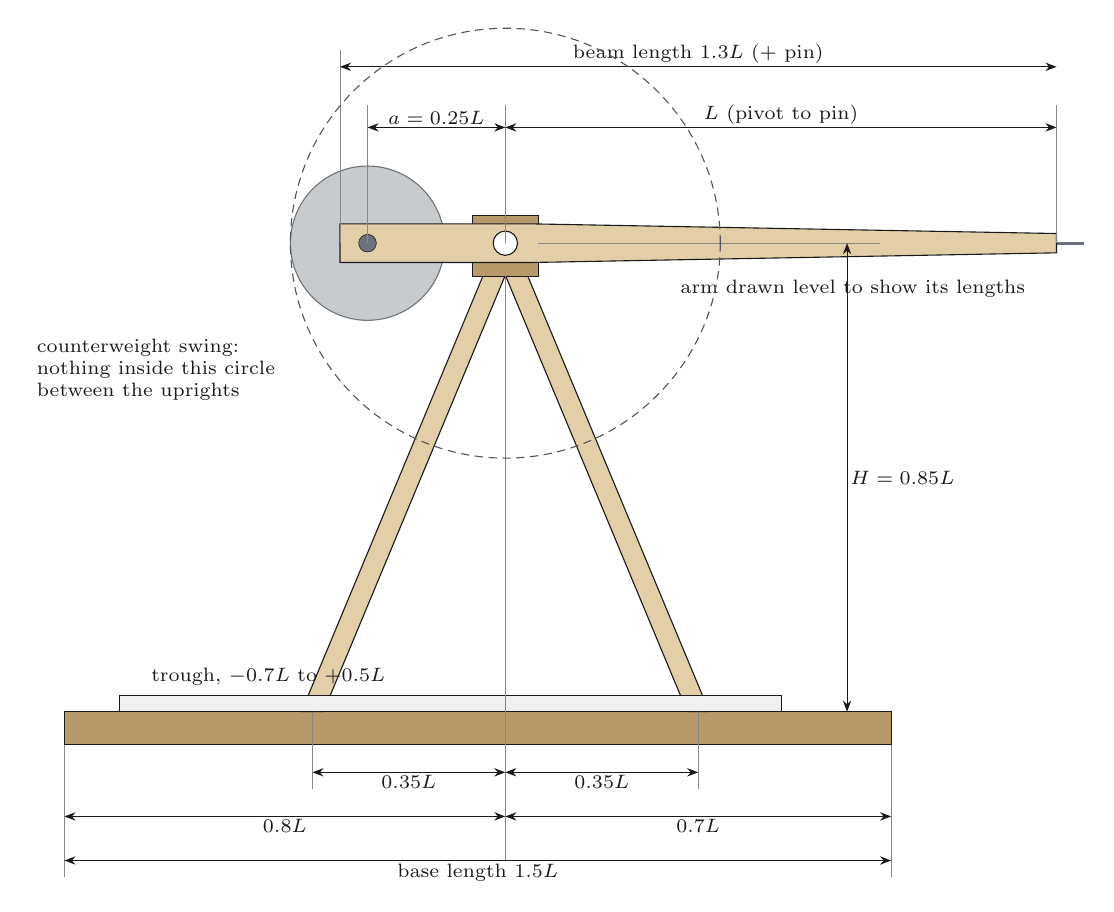
\begin{tikzpicture}[x=7cm, y=7cm]
  \pic at (0,0) {frame};
  % arm resting at rest (counterweight down) for dimensioning: draw horizontal for clarity
  \begin{scope}[shift={(0,0.85)}]
    \fill[Plate, opacity=0.55, draw=Ink, thin] (-0.25,0) circle (0.14);
    \fill[Wood, draw=Ink, thin] (-0.30,-0.035) -- (0.05,-0.035) -- (1.0,-0.0175) -- (1.0,0.0175) -- (0.05,0.035) -- (-0.30,0.035) -- cycle;
    \fill[Steel, draw=Ink, very thin] (-0.25,0) circle (0.016);
    \draw[Steel, line width=1.1pt] (1.0,0) -- (1.05,0);
    \fill[white, draw=Ink, thin] (0,0) circle (0.022);
  \end{scope}
  \node[lbl, anchor=north west] at (0.30,0.80) {arm drawn level to show its lengths};
  % horizontal dims on arm
  \draw[ext] (-0.25,0.85) -- (-0.25,1.10);
  \draw[ext] (0,0.85) -- (0,1.10);
  \draw[ext] (1.0,0.85) -- (1.0,1.10);
  \draw[ext] (-0.30,0.85) -- (-0.30,1.20);
  \draw[dim] (-0.25,1.06) -- (0,1.06) node[midway, above, dl] {$a = 0.25L$};
  \draw[dim] (0,1.06) -- (1.0,1.06) node[midway, above, dl] {$L$ (pivot to pin)};
  \draw[dim] (-0.30,1.17) -- (1.0,1.17) node[midway, above, dl] {beam length $1.3L$ (+ pin)};
  % pivot height
  \draw[ext] (0.06,0.85) -- (0.68,0.85);
  \draw[dim] (0.62,0) -- (0.62,0.85) node[midway, right, dl] {$H = 0.85L$};
  % base length
  \draw[ext] (-0.80,-0.06) -- (-0.80,-0.30);
  \draw[ext] (0.70,-0.06) -- (0.70,-0.30);
  \draw[ext] (0,0.79) -- (0,-0.30);
  \draw[ext] (-0.35,0) -- (-0.35,-0.14);
  \draw[ext] (0.35,0) -- (0.35,-0.14);
  \draw[dim] (-0.35,-0.11) -- (0,-0.11) node[midway, below, dl] {$0.35L$};
  \draw[dim] (0,-0.11) -- (0.35,-0.11) node[midway, below, dl] {$0.35L$};
  \draw[dim] (-0.80,-0.19) -- (0,-0.19) node[midway, below, dl] {$0.8L$};
  \draw[dim] (0,-0.19) -- (0.70,-0.19) node[midway, below, dl] {$0.7L$};
  \draw[dim] (-0.80,-0.27) -- (0.70,-0.27) node[pos=0.5, below, dl] {base length $1.5L$};
  % trough
  \node[lbl, anchor=south] at (-0.43,0.03) {trough, $-0.7L$ to $+0.5L$};
  % counterweight swing clearance
  \draw[densely dashed, LineGrey] (0,0.85) circle (0.39);
  \node[lbl, anchor=east] at (-0.40,0.62) {counterweight swing:\\nothing inside this circle\\between the uprights};
\end{tikzpicture}
\end{center}

\begin{minipage}[t]{0.47\linewidth}
\sechead{Front view}
\begin{center}
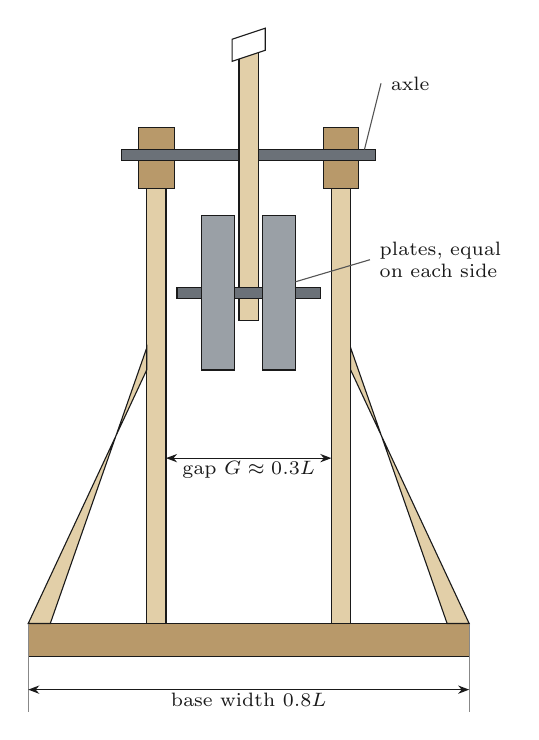
\begin{tikzpicture}[x=7cm, y=7cm]
  % base rails end-on and cross member
  \fill[WoodDark, draw=Ink, thin] (-0.40,-0.06) rectangle (0.40,0);
  % uprights edge-on
  \fill[Wood, draw=Ink, thin] (-0.185,0) rectangle (-0.150,0.84);
  \fill[Wood, draw=Ink, thin] (0.150,0) rectangle (0.185,0.84);
  % side braces
  \draw[Ink, fill=Wood, thin] (-0.185,0.50) -- (-0.185,0.46) -- (-0.40,0) -- (-0.36,0) -- cycle;
  \draw[Ink, fill=Wood, thin] (0.185,0.50) -- (0.185,0.46) -- (0.40,0) -- (0.36,0) -- cycle;
  % bearing blocks
  \fill[WoodDark, draw=Ink, thin] (-0.20,0.79) rectangle (-0.135,0.90);
  \fill[WoodDark, draw=Ink, thin] (0.135,0.79) rectangle (0.20,0.90);
  % axle
  \fill[Steel, draw=Ink, thin] (-0.23,0.84) rectangle (0.23,0.86);
  % beam, hanging at rest (counterweight down), long arm up, broken
  \fill[Wood, draw=Ink, thin] (-0.0175,0.55) rectangle (0.0175,1.05);
  \draw[Ink, thin, fill=white] (-0.03,1.02) -- (0.03,1.04) -- (0.03,1.08) -- (-0.03,1.06) -- cycle;
  % stub and plates
  \fill[Steel, draw=Ink, thin] (-0.13,0.59) rectangle (0.13,0.61);
  \fill[Plate, draw=Ink, thin] (-0.085,0.46) rectangle (-0.025,0.74);
  \fill[Plate, draw=Ink, thin] (0.025,0.46) rectangle (0.085,0.74);
  % dims
  \draw[dim] (-0.150,0.30) -- (0.150,0.30) node[midway, below, dl] {gap $G \approx 0.3L$};
  \draw[ext] (-0.40,0) -- (-0.40,-0.16);
  \draw[ext] (0.40,0) -- (0.40,-0.16);
  \draw[dim] (-0.40,-0.12) -- (0.40,-0.12) node[midway, below, dl] {base width $0.8L$};
  \node[lbl, anchor=west] (p) at (0.22,0.66) {plates, equal\\on each side};
  \draw[lead] (p.west) -- (0.085,0.62);
  \node[lbl, anchor=west] (q) at (0.24,0.98) {axle};
  \draw[lead] (q.west) -- (0.21,0.86);
\end{tikzpicture}
\end{center}
\end{minipage}\hfill
\begin{minipage}[t]{0.50\linewidth}
\sechead{Gap between the uprights}
The counterweight swings \emph{between} the two A-frames, so the inside gap must clear the plates with room to spare:
\[
G = \text{beam width} + 2\times(\text{plate stack} + 40\,\text{mm})
\]
About $0.3L$ suits most builds. Check by swinging the loaded arm slowly through a full turn by hand before you fire.

\sechead{Why these numbers}
They come from a computer model of the trebuchet that includes air resistance and friction. A pivot at $0.85L$ lets the cocked tip rest just above the trough; a $1.5L$ base keeps the frame from tipping as the counterweight falls; the 4\,:\,1 arm and $0.9L$ sling gave the longest throws across all three scales.
\end{minipage}

\newpage
% =====================================================================
%  PAGE 3 -- SIZES AND MATERIALS FOR THREE SCALES
% =====================================================================
\sechead{Sizes for three scales (millimetres)}
{\footnotesize
\begin{tabularx}{\linewidth}{@{}L{3.6cm} L{2.0cm} *{3}{Y}@{}}
\toprule
 & \textbf{Rule} & \textbf{Desktop} & \textbf{Medium} & \textbf{Oval} \\
\midrule
Throwing arm $L$ & $L$ & 400 & 700 & 1000 \\
Short arm $a$ & $0.25L$ & 100 & 175 & 250 \\
Beam length & $1.3L$ & 520 & 910 & 1300 \\
Pivot height $H$ (above base) & $0.85L$ & 340 & 595 & 850 \\
Base length $\times$ width & $1.5L \times 0.8L$ & 600 $\times$ 320 & 1050 $\times$ 560 & 1500 $\times$ 800 \\
Gap between uprights $G$ & $\approx 0.3L$ & 120 & 210 & 300 \\
Legs (4), before trimming & $0.95L$ & 4 $\times$ 380 & 4 $\times$ 665 & 4 $\times$ 950 \\
Sling length $s$ & $0.9L$ & 360 & 630 & 900 \\
Trough & $1.2L$ long & 480 & 840 & 1200 \\
\midrule
Beam timber (on edge) & & 42 $\times$ 19 pine, tapers to 21 deep & 70 $\times$ 19 pine, tapers to 35 deep & 70 $\times$ 35 pine, tapers to 35 deep \\
Target beam mass & $\le \tfrac{1}{7}$ lightest CW & 0.15\,kg & 0.6\,kg & 1.0--1.4\,kg \\
Frame and legs & & 42 $\times$ 19 pine & 42 $\times$ 42 pine & 70 $\times$ 35 pine \\
Base & & 12\,mm plywood & 70 $\times$ 35 pine & 90 $\times$ 45 pine \\
Axle & & 8\,mm steel rod & 12\,mm steel rod & 20\,mm bright steel \\
Bearings & & nylon washers in a snug hole & 12\,mm bronze bushes & 2 $\times$ 20\,mm pillow blocks (P204) \\
Counterweight stub & & 8\,mm rod + wing nuts & 25\,mm steel bar + collars & 25\,mm steel bar + collars \\
Counterweights & & slotted masses & 1.25--2.5\,kg plates & 2.5--5\,kg plates \\
Fixings & & PVA glue + 8g screws & 10g screws; M8 bolts at the bearings & M10 coach bolts; 10g screws \\
Projectile & & 25\,g beanbag & tennis ball & tennis ball \\
\midrule
\textbf{Counterweight range} & & \textbf{1--2.5\,kg} & \textbf{4--10\,kg} & \textbf{7.5--17.5\,kg} \\
\textbf{Build the frame to take} & $1.2\times$ max & \textbf{3\,kg} & \textbf{12\,kg} & \textbf{20\,kg} \\
\bottomrule
\end{tabularx}}

\sechead{Expected range}
Two figures for each counterweight: \textbf{plan on} is the model's range less 30\% for real-world losses (a stretchy sling, a rough release, a sticky axle); \textbf{best case} is the model with everything tuned. Lay out your range for the best case.

{\footnotesize
\begin{tabularx}{\linewidth}{@{}L{2.3cm} *{3}{Y}@{}}
\toprule
 & \textbf{Desktop} (25\,g beanbag) & \textbf{Medium} (tennis ball) & \textbf{Oval} (tennis ball, 1.4\,kg beam) \\
\midrule
Counterweight $\to$ & plan on / best case & plan on / best case & plan on / best case \\
\midrule
 & 1\,kg: 4 / 6\,m & 4\,kg: 12 / 17\,m & 5\,kg: 12 / 17\,m \\
 & 1.5\,kg: 7 / 11\,m & 6\,kg: 16 / 23\,m & 7.5\,kg: 18 / 25\,m \\
 & 2\,kg: 10 / 14\,m & 8\,kg: 19 / 27\,m & 10\,kg: 21 / 30\,m \\
 & 2.5\,kg: 11 / 16\,m & 10\,kg: 21 / 29\,m & 12.5\,kg: 24 / 34\,m \\
 & & & 15\,kg: 25 / 36\,m \\
 & & & 17.5\,kg: 27 / 38\,m \\
\midrule
Peak arm spin & 7--12\,rad/s (420--660\textdegree/s) & 7--10\,rad/s (400--560\textdegree/s) & 5--9\,rad/s (260--490\textdegree/s) \\
\bottomrule
\end{tabularx}}

\textbf{For a 20\,m minimum on the oval}, use five counterweights from 7.5 to 17.5\,kg in 2.5\,kg steps. The medium scale also reaches 20\,m with 8--10\,kg and is easier to carry, but has less margin.

\sechead{Tools}
Drop saw or hand saw and mitre box; drill with spade or Forstner bits for the axle hole and a drill stand if you have one (the axle holes must be square to the timber); spanners; clamps; tape measure and square; sandpaper; a hand plane or jigsaw for the taper.

\newpage
% =====================================================================
%  PAGES 4-5 -- BUILD STEPS
% =====================================================================
\sechead{Build the frame}

\begin{minipage}[t]{0.50\linewidth}
\step{1}{Base}
Make a rectangle: two side rails $1.5L$ long, joined by three cross members (front, back, and one under the pivot). Mark the \textbf{pivot line} across both rails $0.8L$ from the back. Glue and screw (desktop) or bolt (oval). Check the diagonals are equal so the base is square.

\step{2}{Uprights}
Each side gets an A-frame: two legs from the rail $0.35L$ in front of and behind the pivot line, meeting at a bearing block. Cut the leg tops at the angle where they meet (lay them on the floor over a full-size chalk drawing of the side view --- the easiest way to get the angle right). The axle centre must be at $H = 0.85L$ above the base.

\step{3}{Side braces}
Fit a diagonal brace from each A-frame, about two-thirds of the way up, down to the outside edge of the base. They stop the frame rocking sideways.
\end{minipage}\hfill
\begin{minipage}[t]{0.47\linewidth}
\vspace{4pt}
\begin{center}
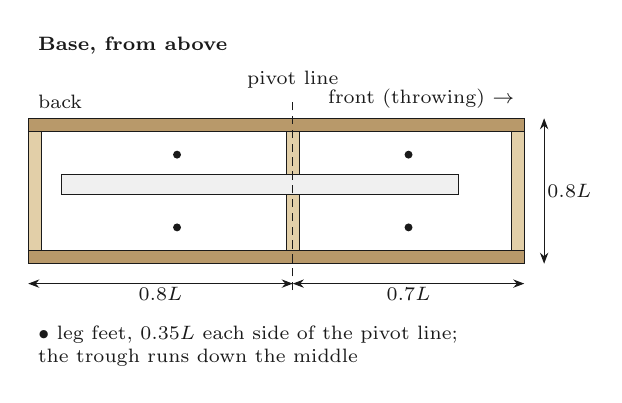
\begin{tikzpicture}[x=4.2cm, y=4.2cm]
  \node[lbl, anchor=west] at (-0.80,0.62) {\bfseries Base, from above};
  % rails
  \fill[WoodDark, draw=Ink, thin] (-0.80,0.36) rectangle (0.70,0.40);
  \fill[WoodDark, draw=Ink, thin] (-0.80,-0.04) rectangle (0.70,0.0);
  % cross members
  \fill[Wood, draw=Ink, thin] (-0.80,0.0) rectangle (-0.76,0.36);
  \fill[Wood, draw=Ink, thin] (0.66,0.0) rectangle (0.70,0.36);
  \fill[Wood, draw=Ink, thin] (-0.02,0.0) rectangle (0.02,0.36);
  % trough
  \fill[BoxGrey, draw=Ink, very thin] (-0.70,0.17) rectangle (0.50,0.23);
  % leg feet
  \foreach \x in {-0.35,0.35}{\fill[Ink] (\x,0.07) circle (0.012); \fill[Ink] (\x,0.29) circle (0.012);}
  \draw[densely dashed, Ink] (0,-0.12) -- (0,0.46) node[above, lbl] {pivot line};
  \draw[dim] (-0.80,-0.10) -- (0,-0.10) node[midway, below, dl] {$0.8L$};
  \draw[dim] (0,-0.10) -- (0.70,-0.10) node[midway, below, dl] {$0.7L$};
  \draw[dim] (0.76,-0.04) -- (0.76,0.40) node[midway, right, dl] {$0.8L$};
  \node[lbl, anchor=north west] at (-0.80,-0.20) {$\bullet$ leg feet, $0.35L$ each side of the pivot line;\\the trough runs down the middle};
  \node[lbl, anchor=south west] at (-0.80,0.40) {back};
  \node[lbl, anchor=south east] at (0.70,0.40) {front (throwing) $\rightarrow$};
\end{tikzpicture}

\vspace{6pt}
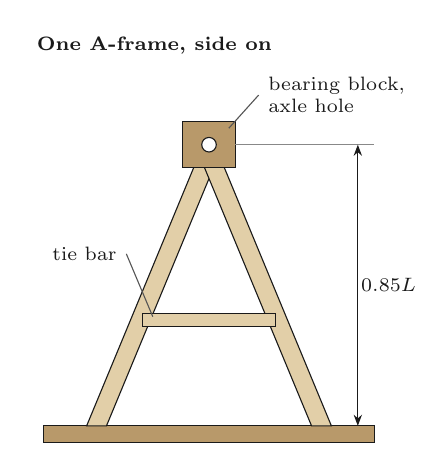
\begin{tikzpicture}[x=4.2cm, y=4.2cm]
  \node[lbl, anchor=west] at (-0.55,1.15) {\bfseries One A-frame, side on};
  \fill[WoodDark, draw=Ink, thin] (-0.50,-0.05) rectangle (0.50,0);
  \draw[Ink, fill=Wood, thin] (-0.37,0) -- (-0.31,0) -- (0.03,0.82) -- (-0.03,0.82) -- cycle;
  \draw[Ink, fill=Wood, thin] (0.31,0) -- (0.37,0) -- (0.03,0.82) -- (-0.03,0.82) -- cycle;
  \fill[Wood, draw=Ink, thin] (-0.20,0.30) rectangle (0.20,0.34);
  \fill[WoodDark, draw=Ink, thin] (-0.08,0.78) rectangle (0.08,0.92);
  \fill[white, draw=Ink] (0,0.85) circle (0.022);
  \draw[ext] (0.08,0.85) -- (0.50,0.85);
  \draw[dim] (0.45,0) -- (0.45,0.85) node[midway, right, dl] {$0.85L$};
  \node[lbl, anchor=west] (bb) at (0.15,1.00) {bearing block,\\axle hole};
  \draw[lead] (bb.west) -- (0.06,0.90);
  \node[lbl, anchor=east] (cr) at (-0.25,0.52) {tie bar};
  \draw[lead] (cr.east) -- (-0.17,0.33);
\end{tikzpicture}
\end{center}
\end{minipage}

\step{4}{Bearings and axle}
Drill the axle holes \textbf{after} both A-frames are fixed, through both bearing blocks in one line (use a long drill bit, or clamp a straight-edge across both blocks). On the oval scale, bolt a pillow-block bearing on top of each block instead and shim them level. The axle must turn freely: spin it by hand --- it should keep turning.

\sechead{Build the arm}
\begin{center}
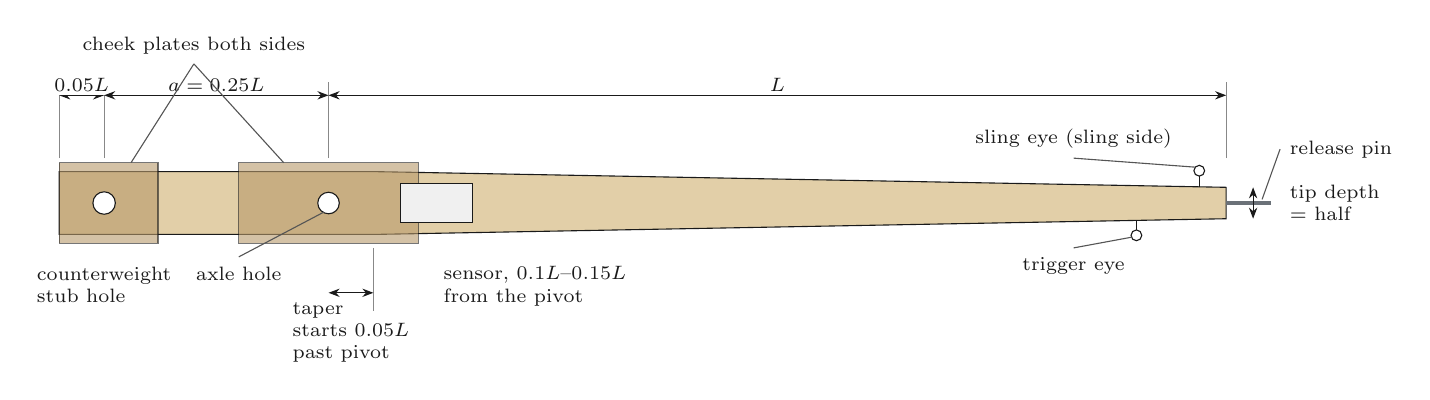
\begin{tikzpicture}[x=11.4cm, y=11.4cm]
  % beam, horizontal, CW end at left
  \fill[Wood, draw=Ink, thin] (0,-0.035) -- (0.35,-0.035) -- (1.30,-0.0175) -- (1.30,0.0175) -- (0.35,0.035) -- (0,0.035) -- cycle;
  % cheek plates
  \fill[WoodDark, opacity=0.6, draw=Ink, thin] (0.20,-0.045) rectangle (0.40,0.045);
  \fill[WoodDark, opacity=0.6, draw=Ink, thin] (0.0,-0.045) rectangle (0.11,0.045);
  % holes
  \fill[white, draw=Ink, thin] (0.30,0) circle (0.012);
  \fill[white, draw=Ink, thin] (0.05,0) circle (0.0125);
  % pin
  \draw[Steel, line width=1.4pt] (1.30,0) -- (1.35,0);
  % eye screws
  \draw[Ink, thin] (1.27,0.0175) -- (1.27,0.03); \draw[Ink, thin] (1.27,0.036) circle (0.006);
  \draw[Ink, thin] (1.20,-0.019) -- (1.20,-0.03); \draw[Ink, thin] (1.20,-0.036) circle (0.006);
  % sensor
  \fill[BoxGrey, draw=Ink, thin] (0.38,-0.022) rectangle (0.46,0.022);
  % dims
  \foreach \x in {0,0.05,0.30,1.30}{\draw[ext] (\x,0.05) -- (\x,0.135);}
  \draw[dim] (0,0.12) -- (0.05,0.12) node[midway, above, dl] {$0.05L$};
  \draw[dim] (0.05,0.12) -- (0.30,0.12) node[midway, above, dl] {$a = 0.25L$};
  \draw[dim] (0.30,0.12) -- (1.30,0.12) node[midway, above, dl] {$L$};
  \draw[ext] (0.35,-0.05) -- (0.35,-0.12);
  \draw[dim] (0.30,-0.10) -- (0.35,-0.10);
  \node[lbl, anchor=north] at (0.325,-0.10) {taper\\starts $0.05L$\\past pivot};
  \draw[dim] (1.33,-0.0175) -- (1.33,0.0175);
  \node[lbl, anchor=west] at (1.36,0) {tip depth\\= half};
  % labels
  \node[lbl, anchor=north] (h1) at (0.05,-0.06) {counterweight\\stub hole};
  \node[lbl, anchor=north] (h2) at (0.20,-0.06) {axle hole};
  \draw[lead] (0.20,-0.06) -- (0.295,-0.01);
  \node[lbl, anchor=north] at (0.53,-0.06) {sensor, $0.1L$--$0.15L$\\from the pivot};
  \node[lbl, anchor=south] at (1.13,0.05) {sling eye (sling side)};
  \draw[lead] (1.13,0.05) -- (1.265,0.04);
  \node[lbl, anchor=north] at (1.13,-0.05) {trigger eye};
  \draw[lead] (1.13,-0.05) -- (1.195,-0.038);
  \node[lbl, anchor=south] at (0.15,0.155) {cheek plates both sides};
  \draw[lead] (0.15,0.155) -- (0.25,0.045);
  \draw[lead] (0.15,0.155) -- (0.08,0.045);
  \node[lbl, anchor=west] at (1.36,0.06) {release pin};
  \draw[lead] (1.36,0.06) -- (1.34,0.004);
\end{tikzpicture}
\end{center}

\step{5}{Cut and taper the beam}
Cut the beam $1.3L$ long. Mark the axle hole $0.30L$ from the counterweight end and the stub hole $0.05L$ from it. From $0.05L$ past the axle hole, plane or saw a straight taper on the \emph{underside} so the tip is half the full depth. Weigh it: aim for the target mass on page~3.

\step{6}{Cheek plates and holes}
Glue and screw a cheek plate (12\,mm plywood, or 6\,mm aluminium on the oval scale) to \textbf{both} faces around the axle hole and around the stub hole. The holes take all the force; without cheek plates the beam can split along the grain. Drill both holes square through beam and plates together, a sliding fit on the axle and stub.

\step{7}{Fit the arm}
Slide the axle through one bearing, the beam, and the other bearing. Fit spacer washers (or collars on the oval scale) so the beam sits centred in the gap and cannot slide sideways. Push the counterweight stub through its hole and fit collars either side of the beam.

\step{8}{Release pin, eyes and trough}
Drill the tip and fit the release pin --- a bolt with the head cut off, or 6\,mm steel rod --- \textbf{straight out along the line of the arm}, sticking out about $0.05L$. Round and polish its end. Screw an eye into the sling side near the tip ($0.03L$ from the end) and a stronger eye on the other side ($0.1L$ from the end) for the trigger cord. Fix a smooth trough down the centre of the base: half a length of PVC pipe (90\,mm for a tennis ball) or a lined channel.

\sechead{Sling, release pin and trigger}

\begin{minipage}[t]{0.50\linewidth}
\step{9}{Sling and pouch}
Use low-stretch cord (braided polyester, not elastic or nylon rope). Cut two cords each a little over $s = 0.9L$.
\begin{itemize}[itemsep=1pt, leftmargin=1.2em, topsep=1pt]
  \item The \textbf{fixed cord} is tied to the sling eye.
  \item The \textbf{release cord} ends in a small steel ring that drops loosely over the release pin.
  \item The \textbf{pouch} is a rectangle of canvas or leather about $3\times$ by $2\times$ the ball's diameter, with a hole at each end for the cords. A small hole in the middle stops it cupping air.
\end{itemize}
Measure $s$ from the tip of the arm to the centre of the pouch with both cords pulled straight. Both cords must be exactly the same length or the ball will fly off to one side.
\end{minipage}\hfill
\begin{minipage}[t]{0.47\linewidth}
\vspace{2pt}
\begin{center}
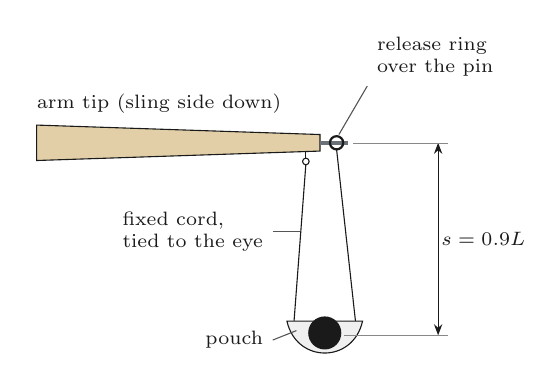
\begin{tikzpicture}[x=6cm, y=6cm]
  \fill[Wood, draw=Ink, thin] (-0.60,0.40) -- (0,0.42) -- (0,0.455) -- (-0.60,0.475) -- cycle;
  \draw[Steel, line width=1.4pt] (0,0.4375) -- (0.06,0.4375);
  \draw[Ink, thin] (-0.03,0.42) -- (-0.03,0.405); \draw[Ink, thin] (-0.03,0.398) circle (0.007);
  % release ring on pin
  \draw[Ink, thick] (0.035,0.4375) circle (0.014);
  % cords to pouch
  \draw[Ink, thin] (-0.03,0.392) -- (-0.055,0.06);
  \draw[Ink, thin] (0.035,0.424) -- (0.075,0.06);
  % pouch
  \draw[Ink, fill=BoxGrey, thin] (-0.07,0.06) .. controls (-0.05,-0.03) and (0.07,-0.03) .. (0.09,0.06) -- cycle;
  \fill[Ink] (0.01,0.035) circle (0.035);
  \draw[dim] (0.25,0.4375) -- (0.25,0.03) node[midway, right, dl] {$s = 0.9L$};
  \draw[ext] (0.07,0.4375) -- (0.27,0.4375);
  \draw[ext] (0.05,0.03) -- (0.27,0.03);
  \node[lbl, anchor=east] (fc) at (-0.10,0.25) {fixed cord,\\tied to the eye};
  \draw[lead] (fc.east) -- (-0.043,0.25);
  \node[lbl, anchor=west] (rc) at (0.10,0.62) {release ring\\over the pin};
  \draw[lead] (rc.south west) -- (0.04,0.455);
  \node[lbl, anchor=east] (po) at (-0.10,0.02) {pouch};
  \draw[lead] (po.east) -- (-0.05,0.04);
  \node[lbl, anchor=west] at (-0.62,0.52) {arm tip (sling side down)};
\end{tikzpicture}
\end{center}
\end{minipage}

\begin{minipage}[t]{0.50\linewidth}
\step{10}{Set the release pin}
The pin decides \emph{when} the ring slides off, and so the angle the ball leaves at. Start with it \textbf{straight}, along the line of the arm. Tune it later by bending it a little at a time (page~6):
\begin{itemize}[itemsep=1pt, leftmargin=1.2em, topsep=1pt]
  \item bend it \textbf{towards the sling side} $\to$ the ring slides off \textbf{earlier} $\to$ a higher throw;
  \item bend it \textbf{away from the sling side} $\to$ \textbf{later} $\to$ a lower, flatter throw.
\end{itemize}
Change it 5--10\textdegree{} at a time. Never bend it so far towards the sling side that the ring can slide off while the arm is cocked.
\end{minipage}\hfill
\begin{minipage}[t]{0.47\linewidth}
\vspace{2pt}
\begin{center}
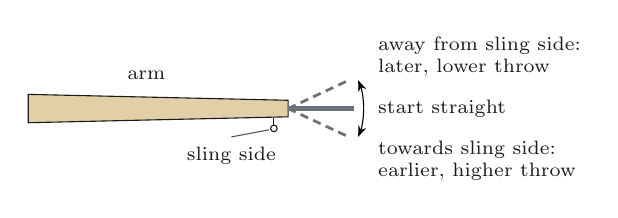
\begin{tikzpicture}[x=6cm, y=6cm]
  \fill[Wood, draw=Ink, thin] (-0.55,-0.03) -- (0,-0.0175) -- (0,0.0175) -- (-0.55,0.03) -- cycle;
  \draw[Steel, line width=1.6pt] (0,0) -- (0.14,0);
  \draw[Steel, line width=1.0pt, densely dashed] (0,0) -- (25:0.14);
  \draw[Steel, line width=1.0pt, densely dashed] (0,0) -- (-25:0.14);
  \draw[-{Stealth[length=4pt]}, thin] (0.16,0) arc[start angle=0, end angle=22, radius=0.16];
  \draw[-{Stealth[length=4pt]}, thin] (0.16,0) arc[start angle=0, end angle=-22, radius=0.16];
  \node[lbl, anchor=west] at (0.17,0.11) {away from sling side:\\later, lower throw};
  \node[lbl, anchor=west] at (0.17,-0.11) {towards sling side:\\earlier, higher throw};
  \node[lbl, anchor=west] at (0.17,0) {start straight};
  \draw[Ink, thin] (-0.03,-0.019) -- (-0.03,-0.035); \draw[Ink, thin] (-0.03,-0.042) circle (0.007);
  \node[lbl, anchor=north] at (-0.12,-0.06) {sling side};
  \draw[lead] (-0.12,-0.06) -- (-0.04,-0.045);
  \node[lbl, anchor=south] at (-0.30,0.04) {arm};
\end{tikzpicture}
\end{center}
\end{minipage}

\step{11}{Trigger and safety strap}
\begin{minipage}[t]{0.50\linewidth}
Fix two eye bolts close together on the back cross member, under where the trigger eye on the arm sits when cocked. A short loop of strong cord from the arm's trigger eye passes between them, and a steel pin (a 10\,mm bolt or clevis pin) slides through both eyes and the loop. Tie a 3--4\,m \textbf{pull cord} to the pin so the operator fires from the side, behind the 0\,m line.

Add a \textbf{safety strap}: a second loop from the arm to the base, closed with a carabiner. It goes on before anyone loads and comes off last, once everyone is clear.

On the desktop scale a finger on the arm or a cotter pin is enough.
\end{minipage}\hfill
\begin{minipage}[t]{0.47\linewidth}
\vspace{-6pt}
\begin{center}
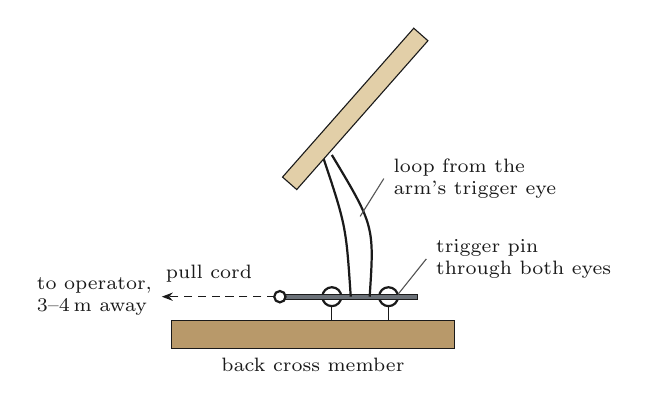
\begin{tikzpicture}[x=6cm, y=6cm]
  \fill[WoodDark, draw=Ink, thin] (-0.40,-0.06) rectangle (0.20,0);
  % eye bolts
  \foreach \x in {-0.06,0.06}{\draw[Ink, thin] (\x,0) -- (\x,0.03); \draw[Ink, thick] (\x,0.05) circle (0.02);}
  % pin through eyes
  \fill[Steel, draw=Ink, very thin] (-0.16,0.045) rectangle (0.12,0.055);
  \draw[Ink, thick] (-0.17,0.05) circle (0.012);
  % loop from arm
  \draw[Ink, thick] (-0.02,0.05) .. controls (-0.03,0.20) .. (-0.08,0.35);
  \draw[Ink, thick] (0.02,0.05) .. controls (0.03,0.20) .. (-0.06,0.35);
  % arm fragment
  \begin{scope}[shift={(-0.07,0.38)}, rotate=228.6]
    \fill[Wood, draw=Ink, thin] (-0.3,-0.02) rectangle (0.12,0.02);
  \end{scope}
  % pull cord
  \draw[Ink, thin, densely dashed, -{Stealth[length=4pt]}] (-0.18,0.05) -- (-0.42,0.05);
  \node[lbl, anchor=south] at (-0.32,0.06) {pull cord};
  \node[lbl, anchor=east] at (-0.42,0.05) {to operator,\\3--4\,m away};
  \node[lbl, anchor=west] (tp) at (0.14,0.13) {trigger pin\\through both eyes};
  \draw[lead] (tp.west) -- (0.08,0.055);
  \node[lbl, anchor=west] (lp) at (0.05,0.30) {loop from the\\arm's trigger eye};
  \draw[lead] (lp.west) -- (0.0,0.22);
  \node[lbl, anchor=north] at (-0.10,-0.06) {back cross member};
\end{tikzpicture}
\end{center}
\end{minipage}

\step{12}{Sensor mount}
\begin{minipage}[t]{0.62\linewidth}
Strap the PASCO sensor to the \textbf{face} of the throwing arm, $0.1L$--$0.15L$ from the axle, with a hook-and-loop strap and a cable tie as backup. Keep it flat and square to the beam so one gyroscope axis lines up with the axle --- that axis then reads the arm's spin directly. Near the pivot the sensor feels little force and barely changes how the arm swings. Check the peak spin on page~3 against the sensor's gyroscope range in SPARKvue before the first launch.
\end{minipage}\hfill
\begin{minipage}[t]{0.34\linewidth}
\vspace{-4pt}
\begin{center}
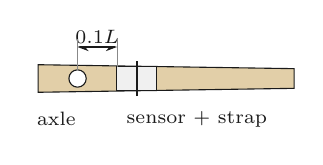
\begin{tikzpicture}[x=5cm, y=5cm]
  \fill[Wood, draw=Ink, thin] (-0.10,-0.035) -- (0.55,-0.025) -- (0.55,0.025) -- (-0.10,0.035) -- cycle;
  \fill[white, draw=Ink, thin] (0,0) circle (0.022);
  \fill[BoxGrey, draw=Ink, thin] (0.10,-0.03) rectangle (0.20,0.03);
  \draw[Ink, thick] (0.15,-0.045) -- (0.15,0.045);
  \draw[dim] (0,0.08) -- (0.10,0.08) node[midway, above, dl] {$0.1L$};
  \draw[ext] (0,0.022) -- (0,0.10); \draw[ext] (0.10,0.03) -- (0.10,0.10);
  \node[lbl, anchor=north west] at (0.10,-0.06) {sensor + strap};
  \node[lbl, anchor=north east] at (0.02,-0.06) {axle};
\end{tikzpicture}
\end{center}
\end{minipage}

\newpage
% =====================================================================
%  PAGE 6 -- COMMISSIONING AND TUNING
% =====================================================================
\sechead{First launches and tuning}
\begin{center}
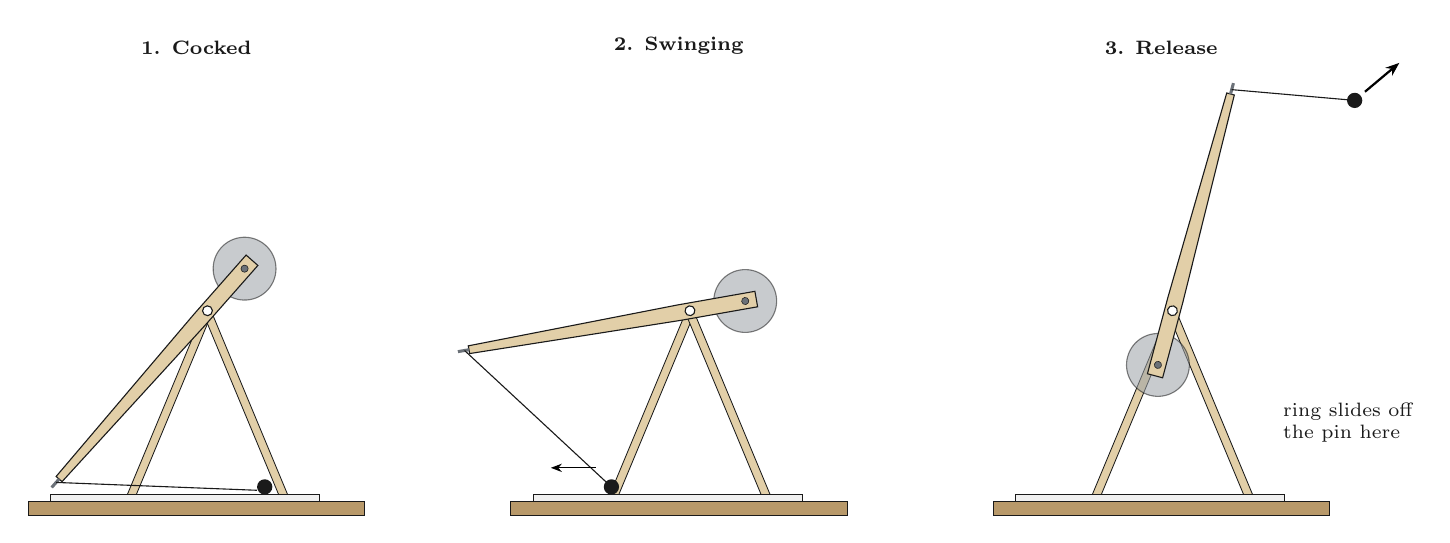
\begin{tikzpicture}[x=2.85cm, y=2.85cm]
  \foreach \px/\ang/\title in {0/228.6/{1. Cocked},2.15/190/{2. Swinging}, 4.3/75/{3. Release}}{
    \begin{scope}[shift={(\px,0)}]
      \fill[WoodDark, draw=Ink, very thin] (-0.80,-0.06) rectangle (0.70,0);
      \draw[Ink, line width=0.3pt, fill=Wood] (-0.37,0) -- (-0.33,0) -- (0.02,0.84) -- (-0.02,0.84) -- cycle;
      \draw[Ink, line width=0.3pt, fill=Wood] (0.33,0) -- (0.37,0) -- (0.02,0.84) -- (-0.02,0.84) -- cycle;
      \fill[BoxGrey, draw=Ink, very thin] (-0.70,0) rectangle (0.50,0.03);
      \pic[rotate=\ang] at (0,0.85) {arm};
      \node[lbl, anchor=south] at (-0.05,1.95) {\bfseries \title};
    \end{scope}}
  % sling 1
  \draw[Ink, thin] ($(0,0.85)+(228.6:1.02)$) -- (0.22,0.05); \fill[Ink] (0.255,0.065) circle (0.034);
  % sling 2: ball dragged along trough
  \draw[Ink, thin] ($(2.15,0.85)+(190:1.02)$) -- (2.15-0.35,0.065); \fill[Ink] (2.15-0.35,0.065) circle (0.034);
  \draw[-{Stealth[length=4pt]}, thin] (2.15-0.42,0.15) -- (2.15-0.62,0.15);
  % sling 3
  \coordinate (T3) at ($(4.3,0.85)+(75:1.02)$);
  \draw[Ink, thin] (T3) -- ++(-5:0.55) coordinate (B3); \fill[Ink] (B3) circle (0.034);
  \draw[-{Stealth[length=5pt]}, thick] ($(B3)+(40:0.06)$) -- ++(40:0.2);
  \node[lbl, anchor=west] at (4.3+0.45,0.35) {ring slides off\\the pin here};
\end{tikzpicture}
\end{center}

\step{A}{Commission it empty, then light}
\begin{enumerate}[itemsep=1pt, leftmargin=1.6em, topsep=1pt]
  \item With no counterweight, swing the arm by hand through a full turn. Nothing should touch; the axle should turn freely.
  \item Load the \textbf{lightest} counterweight (equal plates each side). Swing it slowly by hand with the sling fitted: the pouch should run straight down the trough without catching.
  \item Fire with \textbf{no ball} a couple of times. Watch the sling: the ring should leave the pin cleanly as the arm passes the top.
  \item Fire with the ball. Only increase the counterweight once the lightest one throws straight and at a good angle.
\end{enumerate}

\step{B}{Tune it}
{\footnotesize
\begin{tabularx}{\linewidth}{@{}L{5.2cm} Y@{}}
\toprule
\textbf{What you see} & \textbf{What to change} \\
\midrule
Ball goes very high, straight up, or lands behind & Releases too early: bend the pin \textbf{away from the sling side} (later release). \\
Ball hits the ground in front, or goes very low & Releases too late: bend the pin \textbf{towards the sling side} (earlier release). \\
Ball flies off to one side & Sling cords are different lengths, or the trough is not straight. Even them up. \\
Ball falls out of the pouch early & Pouch too shallow or too wide; make it longer so it wraps the ball. \\
Pouch snags in the trough & Smooth the trough; shorten the sling slightly (try $0.8L$). \\
Arm sluggish, short throws & Beam too heavy (taper it more), stiff axle (clean and grease it), or the sling stretches. \\
Frame rocks or walks & Peg the base down or sandbag it; check the side braces. \\
\bottomrule
\end{tabularx}}

Aim for the ball leaving at about \textbf{35--45\textdegree{}} above level --- slightly flatter than 45\textdegree{} goes furthest once air resistance is counted. Once it is tuned, \textbf{do not touch the pin or sling again} for the whole investigation: they are controlled variables.

\step{C}{Check the build before every session}
Axle collars tight \textbullet{} cheek plate screws tight, no cracks near the holes \textbullet{} sling cords not frayed, ring not bent \textbullet{} plates and collars locked on the stub \textbullet{} trigger pin slides freely \textbullet{} base pegged or sandbagged.

\newpage
% =====================================================================
%  PAGE 7 -- SAFETY AND SETTING OUT THE OVAL
% =====================================================================
\sechead{Safety}
\warnbox{\textbf{The counterweight is the main hazard, not the ball.} On the oval scale, 15\,kg falling half a metre can crush a hand or foot. The arm swings back and forth several times after each launch and does not stop by itself quickly.}

\begin{minipage}[t]{0.48\linewidth}
\textbf{Loading and firing}
\begin{enumerate}[itemsep=1pt, leftmargin=1.5em, topsep=1pt]
  \item Change plates \textbf{only} with the arm hanging at rest and the safety strap on. Two people for anything over 10\,kg.
  \item Cock the arm with the safety strap on, then fit the trigger loop and pin.
  \item Load the ball. Everyone except the operator steps back behind the line.
  \item Teacher checks the range is clear and calls ``Range clear''.
  \item Remove the safety strap. Operator calls ``Firing'' and pulls the cord from the side.
  \item Nobody approaches until the arm has \textbf{completely stopped}. Re-fit the safety strap first.
\end{enumerate}
\end{minipage}\hfill
\begin{minipage}[t]{0.48\linewidth}
\textbf{People and equipment}
\begin{itemize}[itemsep=1pt, leftmargin=1.2em, topsep=1pt]
  \item Exclusion zone: a circle of radius $2L + 2$\,m around the trebuchet (4\,m on the oval scale). Mark it with cones.
  \item Nobody in front of the trebuchet or inside the range corridor while it is cocked.
  \item Safety glasses for everyone near the trebuchet.
  \item Tennis balls or beanbags only --- never hard balls or stones.
  \item The trebuchet is never left cocked or loaded unattended.
  \item Retrieve balls only on the teacher's ``All clear'', after the safety strap is back on.
\end{itemize}
\end{minipage}

\sechead{Setting out the oval (oval scale)}
\begin{center}
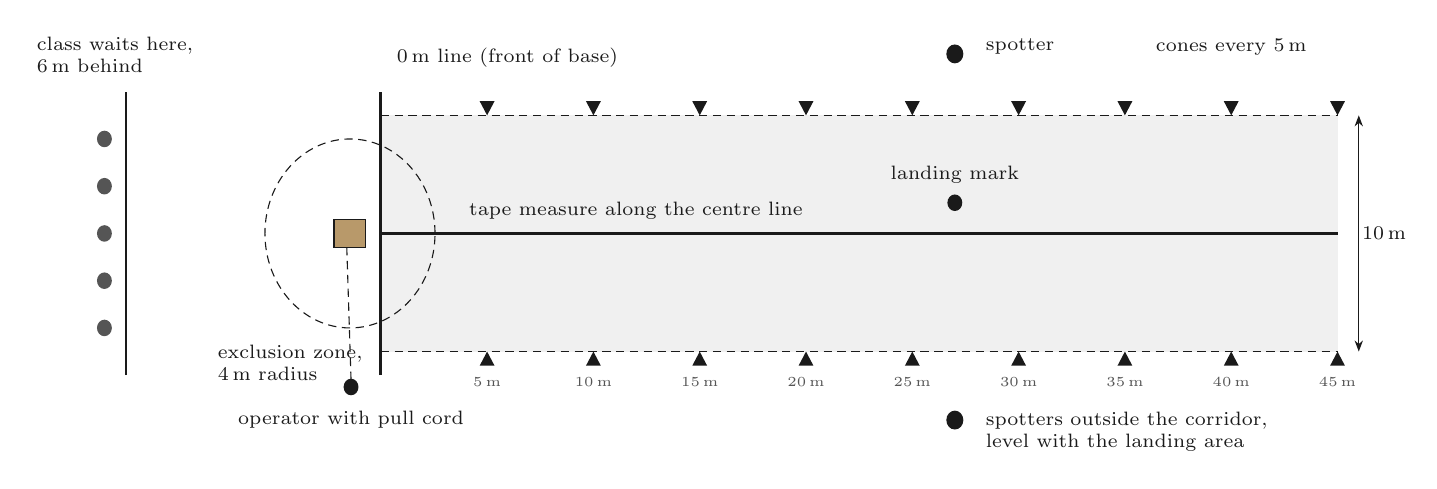
\begin{tikzpicture}[x=0.27cm, y=0.30cm]
  % corridor
  \fill[BoxGrey] (0,-5) rectangle (45,5);
  \draw[Ink, thin, densely dashed] (0,-5) -- (45,-5);
  \draw[Ink, thin, densely dashed] (0,5) -- (45,5);
  % distance ticks / cones every 5 m
  \foreach \x in {5,10,...,45}{
    \fill[Ink] (\x,-5) -- ++(-0.35,-0.6) -- ++(0.7,0) -- cycle;
    \fill[Ink] (\x,5) -- ++(-0.35,0.6) -- ++(0.7,0) -- cycle;
    \node[font=\tiny, text=LineGrey] at (\x,-6.3) {\x\,m};}
  % 0 m line
  \draw[Ink, very thick] (0,-6) -- (0,6);
  \node[lbl, anchor=south west] at (0.3,6.6) {0\,m line (front of base)};
  % trebuchet
  \fill[WoodDark, draw=Ink] (-2.2,-0.6) rectangle (-0.7,0.6);
  \draw[Ink, densely dashed] (-1.45,0) circle (4);
  \node[lbl, anchor=north east] at (-0.4,-4.3) {exclusion zone,\\4\,m radius};
  % tape
  \draw[Ink, thick] (0,0) -- (45,0);
  \node[lbl, anchor=south] at (12,0.2) {tape measure along the centre line};
  % operator
  \fill[Ink] (-1.4,-6.5) circle (0.35);
  \draw[Ink, thin, densely dashed] (-1.4,-6.2) -- (-1.6,-0.6);
  \node[lbl, anchor=north] at (-1.4,-7.1) {operator with pull cord};
  % spectators
  \draw[Ink, thick] (-12,-6) -- (-12,6);
  \foreach \y in {-4,-2,...,4}{\fill[LineGrey] (-13,\y) circle (0.35);}
  \node[lbl, anchor=south] at (-12.5,6.4) {class waits here,\\6\,m behind};
  % spotters
  \foreach \x/\y in {27/7.6,27/-7.9}{\fill[Ink] (\x,\y) circle (0.4);}
  \node[lbl, anchor=west] at (28,-8.4) {spotters outside the corridor,\\level with the landing area};
  \node[lbl, anchor=west] at (28,7.9) {spotter};
  % landing
  \fill[Ink] (27,1.3) circle (0.35);
  \node[lbl, anchor=south] at (27,1.7) {landing mark};
  \draw[dim] (46,-5) -- (46,5) node[midway, right, dl] {10\,m};
  \node[lbl, anchor=west] at (36,7.9) {cones every 5\,m};
\end{tikzpicture}
\end{center}
\vspace{-2pt}
Choose a flat area with the wind \textbf{behind or across} the throw, and make the corridor at least 10\,m wider each side if the wind is gusty. Spotters stand side-on, outside the corridor, and never walk in until the teacher calls ``All clear''. Mark where the ball \textbf{first} lands with a cone or peg, then measure from the 0\,m line along the tape, at right angles to it.

\end{document}
